% calculus:x16 GDC:YES
\begin{question}
  \hspace*{\fill} [Note maximale: 15]\par
  \medskip
  \noindent Une particule $P$ se déplace le long d’une droite. Le vecteur vitesse $v$ $ms^{-1}$ de $P$ après $t$ secondes est donnée par $v(t) = 7 cos t - 5t^{cos t}$, pour $0 \le t \le 7$. Le diagramme suivant montre la représentation graphique de $v$.\par
  \medskip
  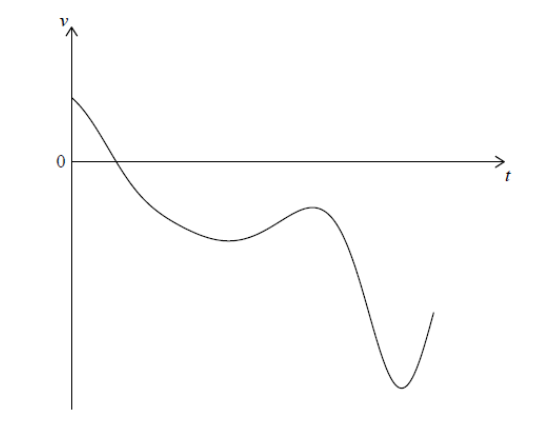
\includegraphics[scale=0.3]{temp_graph_v_vs_t}\par
  \medskip
  (a) Trouvez le vecteur vitesse initiale de $P$.\hspace*{\fill} [2]\par
  \medskip
  (b) Trouvez la vitesse maximale de $P$.\hspace*{\fill} [3]\par
  \medskip
  (c) Écrivez le nombre de fois où l’accélération de $P$ est $0$ $ms^{-2}.$\hspace*{\fill} [3]\par
  \medskip
  (d) Trouvez l’accélération de $P$ lorsque la particule change de direction.\hspace*{\fill} [4]\par
  \medskip
  (e) Trouvez la distance totale parcourue par $P$.\hspace*{\fill} [3]\par
\end{question}

